\chapter{Einleitung}
\section{Ausgangssituation}
Der Energiebedarf ist in den letzen Jahren ständig gewachsen und wird voraussichtlich um 54~\% von 383 EJ in Jahr 2001 auf 591 EJ in Jahr 2025 zunehmen. Zur Deckung dieser Nachfrage bei gleichzeitiger Verminderung der Umweltbelastung durch den anthropogenen  CO2-Anteil in der Atmosphäre, der durch den Verbrauch von fossilen Brennstoffen\index{fossile Brennstoffe} freigesetzt wird, ist Biomasse als Energiequelle von Bedeutung.\footnote{Eine Fußnote}
Biomasse ist in großen Mengen vorhanden. Daher kann die Abhängigkeit von den Erdölproduzenten vermindert werden. Außerdem kann die Energie aus Biomasse wirtschaftlich im Energiemarkt, der aktuell von hohen Erdölpreisen gekennzeichnet ist, wettbewerbsfähig sein .

Die in Biomasse\index{Biomasse} enthaltene Energie kann durch verschiedene Verfahren gewonnen werden und ist CO2-neutral. Umwandlungsverfahren zur Energiegewinnung aus Biomasse werden auf biologischen, physikalischen und thermischen Wegen durchgeführt. Beispiele von Umwandlungsprozessen sind anaerobe Gärung\index{anaerobe Gärung} (Biogasanlage), Verbrennung von Biomasse-Öl hergestellt durch Pyrolyse oder Verflüssigung, Veresterung von pflanzlichen Ölen (Biodiesel), Vergasung und anschließende  Fischer-Tropsch-Synthese\index{Fischer-Tropsch-Synthese}, etc.

Ein Großteil der Restbiomasse fällt als nasses Edukt an. Von allen Alternativen zur Energiegewinnung aus nasser Biomasse (Feuchtigkeit über  40~\%) hat die Vergasung im überkritischen Wasser den höchsten Wirkungsgrad \cite{Yoshi03}, da mit der traditionellen Vergasung bei hohen Wassergehalten aufgrund der nötigen Trocknung der Biomasse nur sehr geringe Wirkungsgrade erzielt werden können. 

Das 21 Jahrhundert ist als die Ära der Gase charakterisiert \cite{Hef02}. Wasserstoff ist das Hauptprodukt der Biomassevergasung in überkritischem Wasser. Durch die Verbrennung von Wasserstoff entsteht nur Wasser als Nebenprodukt. Deshalb ist Wasserstoff aus erneuerbaren Ressourcen, z.B. Biomasse\index{Biomasse}, als der geeignetste und  umweltfreundlichste  Brennstoff in diesem Jahrhundert bewertet worden \cite{Bern03}.

Der kritische Punkt\index{kritischer Punkt} von Wasser liegt bei etwa  374 C und  221 bar. Wasser ist billig, ungiftig und durch Senkung der Temperatur einfach vom Gasprodukt abtrennbar. Eigenschaften wie dielektrische Konstante\index{dielektrische Konstante}, Dichte, etc kann man durch Änderung der Temperatur und des Druckes regulieren. Die Anzahl von Wasserstoffbrücken nimmt bei überkritischen Bedingungen stark ab. Aus diesen Gründen wird die Vergasung von nasser Biomasse in überkritischem Wasser\index{überkritisches Wasser} begünstigt.
Ab 600 C zeigt überkritisches Wasser Oxidationseigenschaften. Sauerstoff vom Wasser reagiert dann mit dem Kohlenstoff der Biomasse hauptsächlich zu CO2 \cite{Feng03}.
Wasserstoff wird sowohl von Wasser als auch von der Biomasse freigesetzt. Die Reaktion ist nicht vollständig; deshalb werden CO, Methan und geringe Mengen anderer Kohlenwasserstoffe gebildet. Die CO-Bildung ist durch die höhere Temperatur unterdrückt, weil die Wasser-Gas-Shift-Reaktion\index{Wasser-Gas-Shift-Reaktion} unter überkritischen Bedingungen begünstigt wird \cite{Sato04}.

Wegen des hohen Prozessdruckes wird durch die Vergasung in überkritischem Wasser Kompressionsarbeit\index{Kompressionsarbeit} für die Speicherung des Gasprodukts gespart. Da die in Biomasse vorhandenen anorganischen Begleitstoffe (K, Na, Si, N, Cl, etc) mit dem Abwasser\index{Abwasser} abgetrennt werden, erfolgt die Gaskonditionierung nur durch Anwendung einer Waschkolonne zur Abtrennung des gebildeten CO2. Damit kann Wasserstoff neben Methan und geringe Mengen höherer Kohlenwasserstoffe in einem einstufigen Verfahren produziert werden. Außerdem wird die Bildung von Teeren und Ruß bei überkritischen Bedingungen unterdrückt. 

Mehrere Berichte über die Vergasung von Modellsubstanzen\index{Modellsubstanzen} sind in der Literatur auffindbar. Lee et al. \cite{Lee02} untersuchten den Einfluss der Temperatur und der Verweilzeit auf die Vergasung von Glucose\index{Glucose} in überkritischem Wasser. Sie fanden, dass die Gasausbeute sehr stark mit steigender Temperatur ab $660 ^{\circ}C$ erhöht wird und in der untersuchten Verweilzeitspanne kein Unterschied in der erzielten Gasausbeute auftrat. Hao et al. \cite{Hao03}  stellten in der Vergasung von Glucose einen vernachlässigbaren Effekt des Druckes fest. Der Effekt der Konzentration wurde bei der Reformierung von Methanol untersucht. Konzentrationserhöhung führte zum Anstieg des CO-Gehalts und zur entsprechenden Abnahme des Wasserstoffanteils im Gasprodukt \cite{tay03}. In der Vergasung von Glucose bei $600 ^{\circ}C$ wurde eine Zunahme der Methankonzentration beobachtet \cite{aih93}.

Der Effekt der Zusammensetzung der Mischungen von Modellsubstanzen wurde auch untersucht. Die Gasausbeute sinkt bei Mischungen, die Lignin enthalten \cite{idea01}, und hängt von der Ligninsorte ab \cite{yoshida04}. Zur Verbesserung der Vergasung von ligninhaltiger Biomasse wurde die Nutzung von Katalysatoren untersucht. Ruthenium-Katalysatoren zeigten eine höhere Aktivität als andere Metalle \cite{sato03}. Osada et al. \cite{osa04} erzielten 30 \% Ligninumsatz bei $400 ^{\circ}C$ an einem Ruthenium-Katalysator. Die Katalysatoren werden in Anwesenheit von Katalysatorgiften wie Schwefel, Chlor, und Metallen deaktiviert \cite{matsu05}. 

Technische Hürden, wie z. B. die Förderung von feststoffhaltigen Edukten mussten vor der Durchführung der Laboruntersuchung mit realer Biomasse überwunden werden. Antal et al. untersuchten zuerst die Vergasung von Biomasse. Sie benutzten Maisstärke als Verdickungsmittel für Biomasse wie Sägemehl und Kartoffelreste. Sie ermittelten vollständige Umsätze bei $700 ^{\circ}C$ mit der Nutzung von Aktivkohle als Katalysator.
 
Im Institut für Technische Chemie, Bereich Chemisch-Physikalische Verfahren, wird dieses Verfahren seit mehreren Jahren erforscht.  Einerseits wird  versucht, den Mechanismus der Vergasung von Biomasse in überkritischem Wasser zu erklären.  Kruse et al.  identifizierten Schlüsselsubstanzen, die in der Vergasung von Glucose in überkritischem Wasser als Intermediaten auftauchen. In neuen Arbeiten wurden die Einflüsse der Aufheizungsrate, der Zugabe von Additiven und der Biomassekonzentration auf die Bildung von Intermediaten untersucht. Der Temperaturbereich dieser Untersuchungen liegt unter $500 ^{\circ}C$. Andererseits werden neuere Reaktorkonzepte zur Optimierung des Verfahren entwickelt. Hochdruckanlagen im Labormaßstab wurden für diesen Zweck entwickelt. Im Jahr 2003 wurde die weltweit einzige Pilot-Anlage mit einem Durchsatz von 100 kg/h in Betrieb genommen. Die Anlage wurde mit den gewonnenen Daten der Vergasung von Modelsubstanzen für die Vergasung von realer Biomasse ausgelegt. 
\section{Aufgabenstellung}
Ziel der vorliegenden Arbeit ist die kinetische Untersuchung und Bewertung der Vergasung von realer Biomasse in überkritischem Wasser mit einer Labor-Hochdruckanlage zum Zweck der Simulation und Optimierung des Verfahrens.

In Rahmen des Projektes ReFuelNet wurde Maissilage als Biomasse für die Untersuchungen ausgewählt.  Maissilage ist ein stabiles Edukt, das über lange Zeiträume abgelagert werden kann. Mais wird weltweit unter vielen klimatischen Bedingungen angebaut.

In der vorliegenden Arbeit wird über den Einfluss der Prozessvariablen  (Temperatur, Druck, Verweilzeit) und der Vorbereitung des Eduktes (Konzentration, Zerkleinerungsgrad, Zusatz von Additiven, Herkunft) auf die Gasausbeute berichtet. Die Versuche wurden zuerst in einem kontinuierlichen horizontalen Rohrreaktor durchgeführt, der zur Verbesserung der erzielten Gasausbeute und zur Verminderung der Feststoffbildung im Rahmen dieser Arbeit modifiziert wurde. 
\chapter{Überkritisches Wasser}
\section{Definition und Bedeutung}
\subsection{Überkritisches Fluid }
Ein Fluid ist \emph{überkritisch}, wenn Druck und Temperatur seine kritischen Werte überschreiten, die durch den sogenannten kritischen Punkt (C) gegeben sind, in dem die Dampfdruckkurve endet. Wenn ein Fluid den kritischen Zustand erreicht hat, ist es nicht mehr möglich, mit Druckerhöhung das Fluid zu verflüssigen. Ab dem kritischen Punkt entsteht ein einphasiger, homogener Bereich, in dem die Stoffeigenschaften zwischen denen der Gas- und Flüssigphase liegen.
Bei einem Druck $p < p_c$  und einer Temperatur von $T < T_c$ ist der Stoff oberhalb der Dampfdruckkurve gasförmig und unterhalb dieser Kurve flüssig. Am Tripelpunkt (TP) stehen alle Aggregatzustännde, d.h Flüssig-, Gas- und Feststoffphase, miteinander im Gleichgewicht.   
Die Eigenschaften eines Fluides sind oberhalb seines kritischen Punkts  deutlich anders als in der Gasphase und hängen zudem stark von Druck und Temperatur ab. Diese Eigenschaften und deren Variabilität erlauben die Entwicklung von neuen Verfahren.

Überkritische Fluide bieten zahlreichende Vorteile gegenüber anderer Lösungsmitteln, weil die Dichten flüssigkeitsähnlich sind. Zudem liegen die für den Stofftransport verantwortlichen Größen wie Viskosität und Diffusionskoeffizienten eher im Bereich von Gasen, was zu einem schnelleren Stofftransport führt. Daher kann die Nutzung von zusätzlichen Lösungsmitteln oder Edukten durch geeignete Wahl der Reaktionsbedingungen in der chemischen Synthese vermieden werden. Beispielsweise ist CO2 ein gutes Lösungsmittel wegen seiner niedrigen kritischen Temperatur in Extraktions- und Kristallisationsprozessen zur Erzeugung von Lebensmitteln und pharmazeutischen Wirkstoffen. Mit der Anwendung von überkritischen Fluiden als Reaktionsmedium können höhere Umsätze erzielt und/oder Verfahrensschritte reduziert werden. Außerdem ist die Abtrennung der überkritischen Fluide vom Produkt durch Druckabbau häufig einfach realisierbar. 

\section{Eigenschaften von Wasser (von Umgebungs- zu überkritischen Bedingungen)}
Wasser, das wichtigste Lösungsmittel in der Natur, zeigt bedeutende Eigenschaften als Reaktionsmedium bei überkritischen Bedingungen, bei denen es sich im Vergleich zu Umgebungsbedingungen anders verhält. In der Natur spielt überkritisches Wasser eine wichtige Rolle in geochemischen Prozessen wie in der Bildung von Mineralvorkommen. 
In der Nähe des kritischen Punkts variieren einige Eigenschaften stark. Die spezifische Wärmekapazität z. B. geht am kritischen Punkt gegen unendlich.  Überkritisches Wasser zeigt eine niedrigere Viskosität, die zu hohen molekularen Schwingungen führt.  Außerdem ermöglicht eine niedrige Viskosität die Kombinierung von hoher Lösungsmitteldichte und schnellem Stofftransport, was diffusionslimitierte Reaktionen beschleunigt. Die Anzahl der Wasserstoffbrücken sinkt bei überkritischen Bedingungen.
Die Dielektrizitätskonstante ($\epsilon$) sinkt mit steigender Temperatur und steigt mit zunehmender Dichte. Bei überkritischem Wasser beträgt $\epsilon$ zwischen 10 und 25, Werte, die typisch für polare Lösungsmittel sind, jedoch nicht so extrem polar wie unter Umgebungsbedingungen ($\epsilon=80$). Damit werden unpolare Substanzen besser gelöst. Die meisten organischen Substanzen können mit überkritischem Wasser gemischt werden.  Die Löslichkeit von unpolaren Gasen wie Sauerstoff und Wasserstoff nimmt mit der Temperatur zu, und oberhalb des kritischen Punktes sind sie vollständig mischbar. Dagegen sinkt die Löslichkeit von Salzen bei überkritischen Bedingungen. Säuren und Basen liegen in überkritischem Wasser weitgehend dissoziiert vor. Zudem werden ionische Substanzen mit steigendem Druck  besser gelöst, was eine Folge zunhemende Dichte.
Das Ionenprodukt $K_w$ steigt bis $10-11$ bei $523,2 K$ und fällt ab auf $10-19$ bei $673,2 K$ und $10-22$ bei $773,2 K$. Wegen der starken Änderung von $\epsilon$ und $K_w$ werden bei Temperaturerhöhung radikalische gegenüber ionischen Reaktionswegen dominant.
\section{Anwendungen des überkritischen Wassers}
In den vergangenen Jahrzehnten sind die Eigenschaften des überkritischen Wassers und dessen Anwendung in chemischen Prozessen  ausführlich untersucht worden. Überkritisches Wasser ist sowohl als Reaktionsmedium wie auch als Edukt von Bedeutung.  
\section{Überkritisches Wasser als Reaktionsmedium}
Das Lösungsvermögen des Wassers ist eine Funktion der Dichte. Bei überkritischen Bedingungen können z.B. Alkane in überkritischem Wasser leicht gelöst werden. Diese Eigenschaft des Wassers führt dazu, dass verschiedene Reaktionen in überkritischem Wasser stattfinden können.

Das SCWO (Supercritical Water Oxidation) Verfahren ist ein Bespiel der Anwendung von überkritischem Wasser als Reaktionsmedium. Organische Schadstoffe beispielweise können mit diesem Verfahren oxidativ abgebaut werden. 

Durch Partialoxidation in überkritischem Wasser können auch schwefelhaltige Kohlenwasserstoffe entschwefelt werden.  

Mit der Anwendung von überkritischem Wasser können Edelmetalle von gebrauchten Katalysatoren wiedergewonnen werden. Aktivkohle kann auch durch Oxidierung in überkritischem Wasser regeneriert werden, da die Schadstoffe desorbiert werden. Auch wird überkritisches Wasser als Co-Lösungsmittel verwendet, z.B. in säure-katalysierten Reaktionen

\section{Überkritisches Wasser als  Reaktant}
Außer für die oben genannten Anwendungen kann überkritisches Wasser auch als Reaktant eingesetzt werden. Wasser ist wegen der verminderten Anzahl  an Wasserstoffbrücken in der Nähe und oberhalb des kritischen Punktes sehr reaktiv; dann kann sich Spaltung oder Hydrolyse der  mit Wasser reagierenden Moleküle ergeben.
 
Von besonderem technischen Interesse ist die Hydrolyse von Nitrilen, Estern und Ethern. Die Hydrolysereaktionen werden häufig durch Zusatz von Säuren katalysiert. In überkritischem Wasser ist ein Katalysatorzusatz häufig überflüssig. Die Reaktionen können wesentlich umweltfreundlicher gestaltet werden. Hydrolyse ist eine sehr effektive Methode zum Abbauen von Kunststoffen, z.B. können Polymere zu wiederverwendbaren Säuren und Glycolen hydrolysiert werden.

\todo{Referenz zu dieser Aussage beifügen}
Überkritisches Wasser kann auch  in  Umlagerungs- oder Eliminierungsreaktionen, die normalerweise sauer katalysiert sind,  einen katalytischen Effekt zeigen. Z.B bei der Herstellung von Perlon tritt die Beckmann-Umlagerung als Zwischenreaktion auf, die in überkritischem Wasser vollständig durchgeführt werden kann. Wasserabspaltung aus Alkoholen ist zum Erzeugen von  Doppelbindungen erwünscht. Die Bildung von tert.-Buten aus tert.-Butanol ist in überkritischem Wasser  mit vollständigem Umsatz möglich

Bei der Behandlung von gebrauchtem Polyurethan mit überkritischem Wasser werden die Monomere abgespalten, die für die weitere Produktion neuer Kunststoffe aus Polyurethan verwendet werden können. Biomasse kann auch in überkritischem Wasser gespalten werden. Das Verfahren der Vergasung von Biomasse in überkritischem Wasser ist Gegenstand der vorliegenden Arbeit und wird im Kapitel III ausführlicher erläutert. 
\begin{figure}[htb]
	\centering
	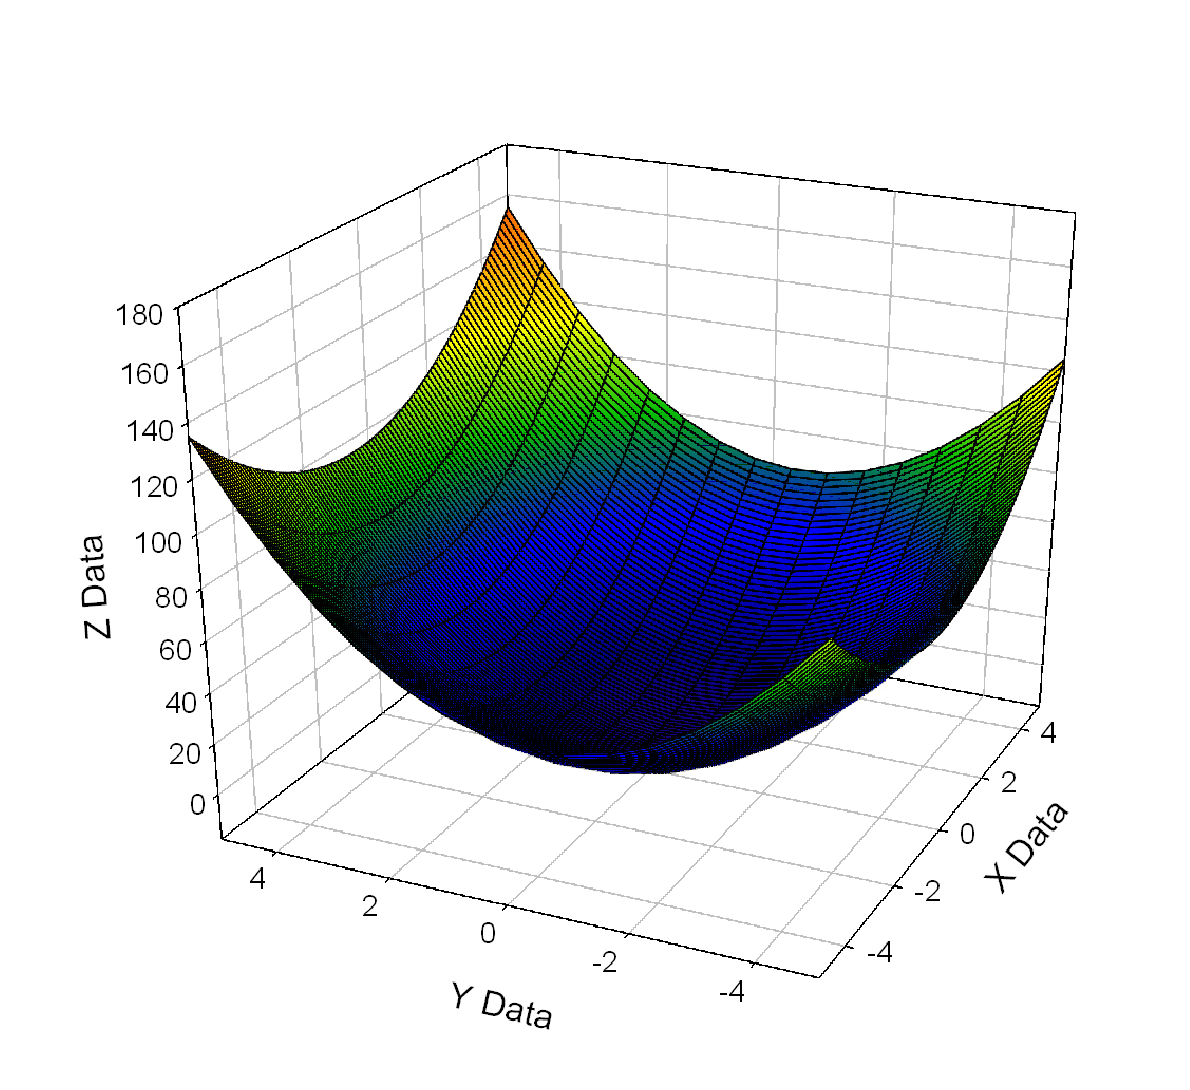
\includegraphics[width=10cm]{graphics/example}
	\caption{Bildunterschriften stehen einheitlich unter den Grafiken.}
\end{figure}
\section{Tabellen}
Die folgende Tabelle soll als Anhaltspunkt dienen. Die Tabelle\index{Tabelle} selbst ist zentriert auszurichten aber sonst individuell formatierbar. Die Verwendung der \emph{table}-Umgebung kann als Gleitumgebung wieder zur Verschiebung der Tabelle führen.
\begin{table}[htb]
	\begin{center}
	\footnotesize
		\begin{tabular}{|l|l|l|l|l|l|}
			\hline
			& $\mathbf{KEA_{fossil}}$ & \multicolumn{4}{c|}{\bfseries{Emissionen}} \\ \hline
			& & $\mathbf{CO}$ & $\mathbf{NO_x}$ & $\mathbf{SO_2}$ & $\mathbf{CO_{2,fossil}}$ \\ \hline
			Einheit & MWh/MWh & kg/MWh & kg/MWh & kg/MWh & kg/MWh \\ \hline
			Steinkohle (D) & 1,06 & 0,010 & 0,046 & 0,062 & 16,9 \\ \hline
			Heizöl EL & 1,11 & 0,035 & 0,107 & 0,182 & 29,5 \\ \hline
			Heizöl S & 1,15 & 0,036 & 0,106 & 0,197 & 38,5 \\ \hline
			Erdgas (D) & 1,07 & 0,050 & 0,045 & 0,047 & 9,85 \\ \hline
		\end{tabular}
	\end{center}
	\label{exampletab}
	\caption{Hier steht eine mögliche Tabellenunterschrift.}
\end{table}
\section{Mathematik-Modus}
Formeln\index{Formeln} werden zentriert geschrieben, wobei die Nummerierung rechtsbündig erfolgt. Durch Einbindung der Pakete \emph{amsmath} und \emph{amssymb} wird der Mathematikmodus\index{Mathematik} von \LaTeXe{} erweitert. 
\begin{equation} 
	\bar{h}(\varphi,x) := \sum_{n\in\mathbb{N}} 2^{-n} \varphi(G_n)^{-1}\mathbf{1}\lbrace x\in G_n \rbrace,
\end{equation}
\begin{equation} 
	\int_{\mathbf{M}(G)}f(\varphi)\mathbb{P}(\mathrm{d}\varphi)=\int_{\mathbf{M}(G)}\int_G h(\theta_{-x}\varphi,x)f(\theta_{-x}\varphi)\mathrm{d}x\mathbb{P}^0(\mathrm{d}\mu)
\end{equation}